%==================================================================%
% Author : Perez Ruiz, Alejandro                                   %
% Version: 1.0, 26/05/2011                                         %                                                                                     % Manual del modelador                                             %
%==================================================================%
\documentclass[a4paper,11pt]{article}

\usepackage[latin1]{inputenc}
\usepackage{url}
\usepackage{amsfonts}
\usepackage[spanish,activeacute]{babel}
\usepackage{graphicx}

\title{User Manual for the creation and configuration of Smart Home models}

\author{Alejandro P�rez \\ Dpto. Matem�ticas, Estad�stica y Computaci�n \\
		Universidad de Cantabria (Santander, Spain)}

\begin{document}

\maketitle

\section{Creating a new project to model and configure smart homes}
To create a new project that allows you to model and create different configurations of smart homes, you must follow the next steps:
\begin{enumerate}
\item Open Visual Studio.
\item Go to \emph{Archive} \ensuremath{\rightarrow} \emph{New...} \ensuremath{\rightarrow} \emph{Project}.
\item In the new window, select the type of project called \emph{Smart Home Project} and click on the \emph{OK} button.
\end{enumerate}

\section{Model and create configurations of smart homes}
To create a model of a smart home, follow the next steps:
\begin{enumerate}
\item In the \emph{Solution Explorer}, doble click on the file called \emph{smartHome.sh}, which it has in the \emph{MyHome} project.
	\begin{center}
			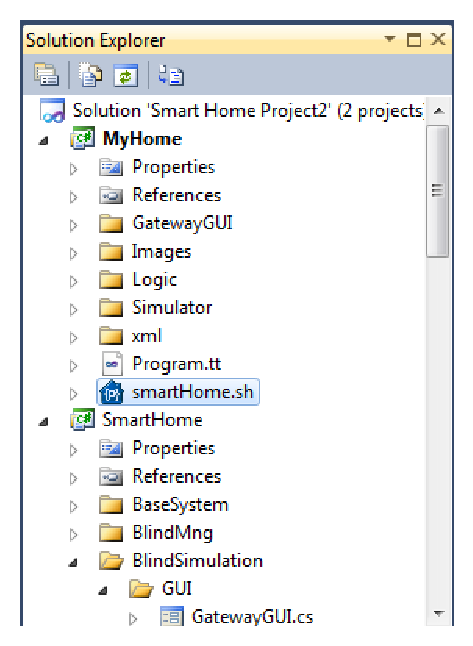
\includegraphics[width=.55\linewidth]{images/solutionExplorer.eps}
			\\
			\vspace{1cm}
	 \end{center}
\item Now, you have a canvas, where you can drag items. The white background of the canvas represents the hole smart home,so everything that you drag in the canvas is a new feature of the smart home. To see the items that you can drag, you must go to the \emph{Toolbox}, if you can't see it, click on \emph{View}-->\ensuremath{\rightarrow}\emph{Toolbox}.
    \begin{center}
			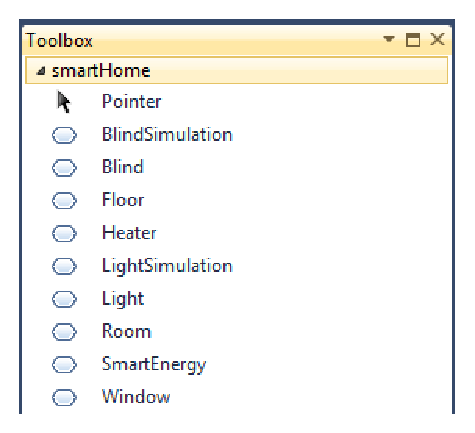
\includegraphics[width=.55\linewidth]{images/toolbox.eps}
			 \vspace{1cm}
	 \end{center}
\item Items that depend on others, such as \emph{Room} needs of a \emph{Floor}, it is necessary to drag the item over which they depend. Thus, the elements \emph{Window}, \emph{Light}, \emph{Heater}, if they want to be added, must be dragged on a room. While a \emph{Blind} must do so on a \emph{Window}.
    \begin{center}
			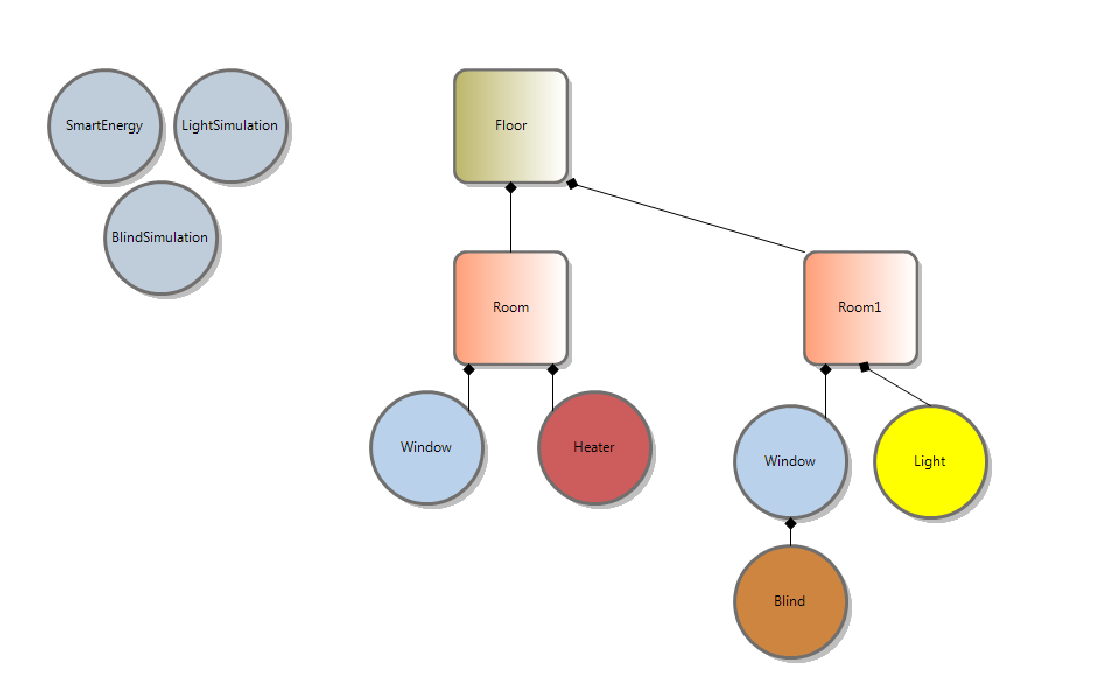
\includegraphics[width=.75\linewidth]{images/exampleSmartHome.eps}
	 \end{center}
\item When the model is ready, save it. To generate the code for the current configuration, go to the \emph{Solution Explorer} and click on the button called \emph{Transform All Templates}.
    \begin{center}
			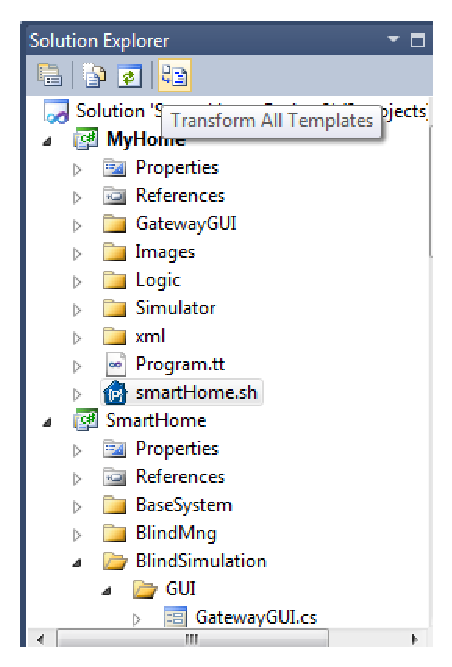
\includegraphics[width=.45\linewidth]{images/transformAllTemplates.eps}
			 \vspace{1cm}
	 \end{center}
\item To execute the current configuration, click with the right button of the mouse on the project called \emph{MyHome} and select \emph{Debug}-->\ensuremath{\rightarrow}\emph{Start New Instance}.
	 \begin{center}
			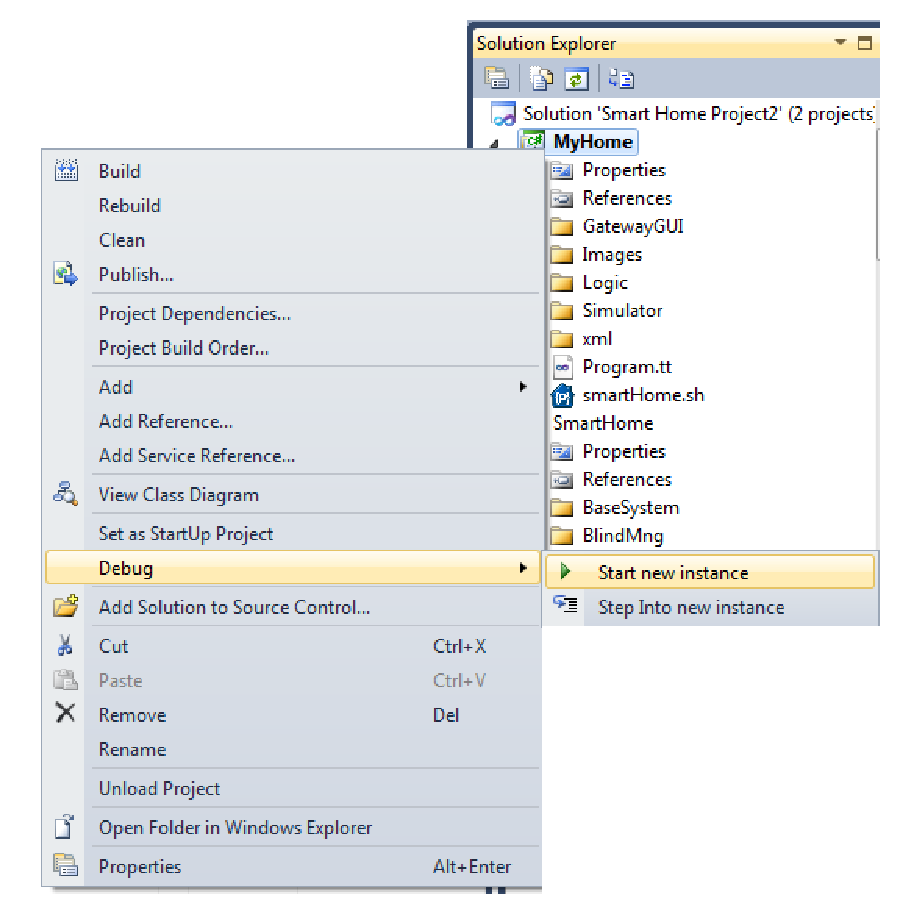
\includegraphics[width=.65\linewidth]{images/startNewInstance.eps}
			 \vspace{1cm}
	 \end{center}
\end{enumerate}

There is a possibility that when you save a configuration, an error alert you. If this happens is because you have violated any of the restrictions contained in a smart home. Thus, you can see the error in the window called \emph{Error List}. For example, if you add the feature \emph{SmartEnergy} without any of the rooms with a heater and a window, you will receive an error.
  \begin{center}
			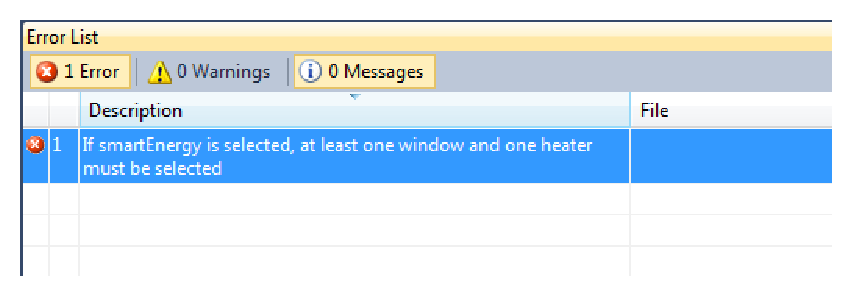
\includegraphics[width=.55\linewidth]{images/error.eps}
			 \vspace{1cm}
  \end{center}
\end{document}
